%%%%%%%%%%%%%%%%%%%%%%%%%%%%%%%%%%%%%%%%%%%%%%%%%%%%%%%%%%%%%%%%%%%%%%%%%%%%%%%
\chapter{基于RAG的方法间变更影响分析}

\section{引言}

由于深度学习模型优秀的泛化能力和知识迁移能力,基于深度学习的变更影响分析方法相较于基于方法间关系的方法具有更优秀的变更影响分析能力。但是由于其性能问题,导致其在实际使用时较为耗时。

为了解决上述问题,本文提出基于RAG的变更影响分析方法,通过训练嵌入模型,将方法代码转换为向量存储,通过检索的方式提高效率,并通过大语言模型进行判断,提高准确率,最后通过实验验证该方法的有效性。

\section{结合依赖路径的数据清洗}



\section{基于RAG的变更影响分析方法}

\subsection{研究方案}

为了解决第二章中深度学习方法的性能问题,本章提出了基于RAG的变更影响分析方法。图中展示了本章方法的研究框架。

本章中的方法主要分为三个阶段。

\begin{itemize}

    \item 数据准备:此阶段的目的生成知识库和收集准确的变更影响关系方法对,用于训练嵌入模型,使嵌入模型只专注于检测变更影响关系的垂直领域。

    \item 检索:将软件代码中的方法组成的集合作为知识库,经过嵌入模型生成向量表示得到向量数据库。被测方法嵌入得到用户向量,在数据库中检索得到候选方法。
    
    \item 增强生成:通过大语言模型对候选方法进行筛选,得到最终的有变更影响关系的方法。
    
\end{itemize}


\subsection{数据准备与编码器训练}

数据准备共有两部分。

\paragraph{生成知识库} 生成知识库是为了方便检索。本方法检索的对象是方法,因此将软件代码按照方法进行分块最为合适。通过第二章中提到的代码预处理得到的抽象语法树,遍历其方法定义节点,得到每个方法的方法体。方法体的集合作为知识库。

\paragraph{编码器数据} 为了使编码器更专注于变更影响关系检测的任务,我们训练嵌入模型,使具有变更影响关系的方法在向量空间中更接近。将研究项目代码通过上章中的四个方法检测得到的有变更影响关系的方法对作为正例进行收集,经过数据清洗得到准确的正例对,并对正例对中任选其一在项目中随机采样得到对应的负例,对应为。独立训练嵌入模型。



编码器训练

考虑到对代码语义的理解能力,这里依旧使用codebert模型作为编码器进行训练。模型的架构如图所示。








\subsection{检索模块}





\subsection{增强模块}




\section{实验结果与分析}

\subsection{实验数据与评价方式}

\subsection{实验结果与对比分析}




\textbf{3.针对于RQ3的实验}

这三种方法检测到的变更影响关系对软件项目的质量贡献如何?应从什么角度指导开发者对软件项目进行维护?

在软件维护过程中,代码变更是必要的,而由于变更影响关系的存在,导致用户在变更时必须谨慎更改,防止功能上和逻辑上的不一致或代码架构的恶化。那么变更影响关系本身是否反映质量问题呢?本文从变更影响关系的数量属性和类型属性进行讨论。

\paragraph{数量属性} 一般而言,一个成熟且高质量的软件项目通常具有清晰的模块化结构,整个软件架构存在模块内高内聚、模块间低耦合的特性,维护起来非常方便。因此对于一个方法而言,如果它的变更会影响到较大的范围,存在“牵一发而动全身”的效应,说明在该方法上可能存在质量问题,从而导致较差的可维护性。

基于上述分析,本章统计了变更影响关系数量位于前 5\% 的方法,认为这些方法可能是代码质量较差的特征代表,并将其作为重点信息报告给用户。统计用户的接受率。得到的结果如表3-8所示。

\begin{table}[htbp]
\caption{变更影响实验结果-接受率}
\vspace{0.5em}\centering\wuhao
\begin{tabular}{ccccc}
\toprule
项目名称 & 依赖闭包 & 克隆代码 & 数据挖掘-支持度2 & 数据挖掘-支持度3 \\
\midrule
TheAlgorithms & 36.2 & \textbf{92.3} & 81.2 & 89.4\\
antiword-0.37 & 33.7 & \textbf{89.9} & - & -\\
jemalloc-5.3.0 & 33.4 & 89.3 & 69.8 & \textbf{92.1}\\
libbpf-1.1 & 40.4 & \textbf{94.4} & 76.4 & 77.3\\
librdkafka-2.1.0 & 28.3 & \textbf{83.7} & 74.3 & 83.2\\
FFmpegKit-5.1.0 & 27.2 & 84.7 & 64.7 & \textbf{87.0}\\

\bottomrule
\end{tabular}
\end{table}

实验结果中,基于依赖闭包的方法的接受率依旧为最低,也就是说,依赖闭包方法检测到的变更影响范围较大的那些方法,并不一定是真实的差质量代码。这同样是由于依赖闭包方法的涟漪效应的不准确性导致的误报问题,这类误报使得大量真实和虚假的变更影响关系混同,导致开发者难以分辨哪些方法是真实的差质量代码,也难以进行变更。在根据代码静态结构得到的变更影响关系中,开发者实际上更信任自己通过阅读代码结构得到的一到二层涟漪效应。

而另外三种方法的效果均优于依赖闭包方法,表明了三种方法提取的关系的数量属性能很好的反映代码的质量。实验结果中有4个项目的最高值均来源于克隆代码方法,即使在最大的数量远低于依赖闭包方法的情况下,仍然能让开发者接受,体现了克隆代码方法的准确性。除此之外,对于克隆代码方法,我们还观察到部分未被接受的方法对存在一些共同的特征,进一步揭示了影响方法准确性的其他因素。例如,以antiword项目中的一对包含克隆代码片段的方法为例,这两个方法的统计信息如表3-6所示,其中克隆代码片段仅占据8行。代码长度的可视化形式以及克隆代码片段如图3-6所示,包含的重复代码仅为两行单独的语句。之所以在统计时被视为克隆代码,主要是由于编程习惯的影响,每个参数被单独放在一行,这导致了克隆代码的扩展至8行。用户认为此例较为牵强,因为克隆代码占整个方法的行数过少,这表明克隆代码所占比例也是开发者决定是否信任该项分析的重要因素之一。

\begin{table}[htbp]
\caption{被用户拒绝实例代码信息}
\vspace{0.5em}\centering\wuhao
\begin{tabular}{cccc}
\toprule
方法 & 代码行数(Line of code)  & 克隆代码长度\\
\midrule
pHdrFtrDecryptor & 125 & 8 \\
szFootnoteDecryptor  & 115 & 8 \\
\bottomrule
\end{tabular}
\end{table}

\begin{figure}[h]
\centering
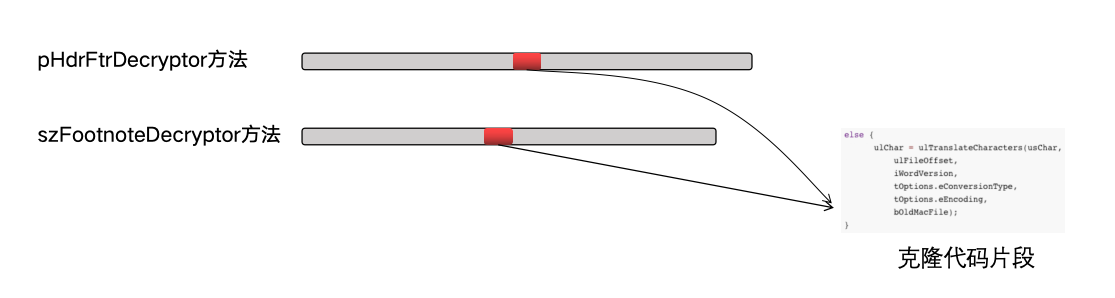
\includegraphics[width = 1.0\textwidth]{克隆代码拒绝样例.jpg}
\caption{被用户拒绝实例代码长度可视化}
\end{figure}

数据挖掘方法的实验结果也高于依赖闭包方法,通过对比支持度不同的实验可以发现,支持度为3略高于支持度为2的接受率,这是由于,支持度为3意味着这对方法起码发生共同修改三次才能被挖掘到,这排除了共同修改2次的方法对的一些偶然情况,挖掘到的关系更少,但是也更为精准。因此,支持度也是决定数据挖掘方法精确度的重要因素之一。

总的来讲,三种方法的数量属性均可以反映质量问题,表现为变更影响范围越大的方法,代码质量越差。在这里我们给到的代码优化和重构建议是,用户可通过合并有变更影响分析的方法或解耦合,从而降低方法的影响关系数量,进而提高代码质量。


\paragraph{类型属性} 本文提出的三种方法中,基于代码克隆方法能检测逻辑型中基于代码克隆的变更影响关系,而基于数据挖掘和基于深度学习的方法能检测更为广泛的逻辑型关系,包括协同方法、镜像方法等。

首先对于代码克隆关系,此种类型的代码在软件项目中一直被认为是较差的代码习惯,主要因为代码克隆通常导致重复性高、维护成本大以及可读性差。代码克隆不仅增加了代码的冗余度,还可能隐藏潜在的缺陷。开发者应使用抽象化的设计模式,通过功能模块化等策略提取重复代码部分,减少重复代码的产生

其次对于


通过对同一软件的不同版本进行检测,得到的实验结果侧面印证了,具有一定的实际应用价值。

\section{本章小结}

本章介绍了四种变更影响分析方法。首先是传统的基于依赖关系闭包的变更影响分析方法。该方法首先对软件项目进行预处理,提取抽象语法树、方法摘要表和全局变量信息表等数据结构,然后构建依赖关系图,节点表示方法和全局变量,边表示方法之间的调用关系。然后根据依赖闭包对每个方法提取对应影响方法。其次是基于克隆代码的变更影响分析方法。该方法认为代码克隆关系一定程度上反映了变更影响关系,通过ClaSP算法进行序列挖掘,提取代码克隆,从而反映变更影响关系。第三种是基于数据挖掘的变更影响分析方法。该方法认为代码变更历史蕴含了一定的变更影响关系,通过提取代码的提交历史,根据频繁模式挖掘理论,挖掘出频繁共现的方法对,从而反映变更影响关系。第四种是基于深度学习的变更影响分析方法。对不存在变更历史的项目,通过数据挖掘得到的数据整理成数据集,训练深度学习模型,对项目方法之间的变更影响关系进行预测。最后,本章通过实验验证了四种方法在提取变更影响关系上的有效性,实验结果表明,除传统的基于依赖关系闭包的方法外,其他方法都取得了良好的检测效果。除此之外还通过实例分析,说明了每种方法的缺点和各自的侧重点。

%%%%%%%%%%%%%%%%%%%%%%%%%%%%%%%%%%%%%%%%%%%%%%%%%%%%%%%%%%%%%%%%%%%%%%%%%%%%%%%